\section{\textsc{Cyder} Repository Modeling Paradigm}

The \Cyder repository model architecture is intended to modularly permit 
exchange of disposal system Component models (e.g., detailed nuclide transport 
model vs. less detailed) and data (e.g., exchange clay for granite geologic 
data) and accept arbitrary waste stream isotopic compositions.  
Finally, in order to participate in the simulation as a facility model, \Cyder must 
make requests for spent material up to its capacity. Determination of the 
repository capacity for various types of spent fuel commodities comprises the 
interfacing functionality of the repository model.

\subsection{Waste Stream Acceptance}

The repository model must accept arbitrary spent fuel and high level waste 
streams. A waste stream is a material data object resulting from the \Cyclus 
simulated fuel cycle.  As radionuclides are gained, lost, and transmuted within 
the spent fuel object, a history of its isotopic composition is recorded.  It 
arrives at the repository and is emplaced if it obeys all repository capacity 
limits. 

For waste streams that vary from each other in composition, the thermal 
capacity of the repository to receive that waste stream must therefore be 
recalculated.  Since disposable material in most simulations of interest will 
be of variable composition and therefore heterogeneous in heat production 
capability, the repository model will repeatedly need to recalculate its own 
capacity as new materials are offered.  That capacity calculation will be 
discussed in Section \ref{sec:thermal_models}. 

\subsection{Waste Stream Conditioning}

Waste conditioning is the process of packing a waste stream into an appropriate 
waste form. As \Cyclus lacks a conditioning facility, the \Cyder repository 
fulfills this need as a part of the repository behavior. As a waste stream is 
accepted into the repository, it is associated with a waste form according 
to its commodity name. This pairing is input by the user during simulation 
setup when a number of waste form Component configurations are specified and 
associated with allowed waste stream commodities. It is according to these 
pairings that \Cyder loads discrete waste forms with discrete waste 
stream contaminant vectors as depicted in Figure \ref{fig:ws_conditioning}.

\begin{figure}[htbp!]
\begin{center}
\def\svgwidth{.5\textwidth}
\input{./chapters/paradigm/ws_conditioning.eps_tex}
\end{center}
\caption[Waste stream conditioning in \Cyder.]{Waste streams are accepted and 
conditioned into the appropriate waste form according to user-specified 
pairings between commodities and waste forms.}
\label{fig:ws_conditioning}
\end{figure}

\subsection{Waste Form Packaging}

Waste packaging is the process of placing one or many waste forms into a 
(typically metallic) containment package. Once the waste stream has been 
conditioned into a waste form, that waste form Component is loaded into a waste 
package Component, also according to allowed pairs dictated by the user, as 
depicted in Figure \ref{fig:wf_packaging}.

\begin{figure}[htbp!]
\begin{center}
\def\svgwidth{.5\textwidth}
\input{./chapters/paradigm/wf_packaging.eps_tex}
\end{center}
\caption[Waste packaging in \Cyder.]{Waste forms are loaded into the 
appropriate waste package according to user-specified pairings between forms 
and packages.}
\label{fig:wf_packaging}
\end{figure}


\subsection{Package Emplacement}

Finally, the waste package is emplaced in a buffer component, which 
contains many other waste packages, spaced evenly in a grid. The grid is 
defined by the user input and depends on repository depth, $\Delta z$, waste 
package spacing, $\Delta x$, and tunnel spacing, $\Delta y$ as in Figure 
\ref{fig:repo_layout}.

\begin{figure}[htbp!]
\begin{center}
\def\svgwidth{.5\textwidth}
\input{./chapters/paradigm/repo_layout.eps_tex}
\end{center}
\caption[The gridded \Cyder repository emplacement geometry.]{The \Cyder 
repository emplacement geometry allows generic representation of all semi-regular 
two dimensional gridded layouts.}
\label{fig:repo_layout}
\end{figure}

\subsection{Nested Components}

The fundamental unit of information in the repository model is radionuclide 
contaminant presence at each stage of containment.  The repository model, in 
this way, is fundamentally a tool to determine thermal and contaminant 
transport evolution as a result of an arbitrary waste stream. The repository 
model in this work conducts this calculation by  treating each containment 
Component as nested volumes in a release chain. 

Each Component is defined by a Geometry, some Material Data, a ThermalModel, 
and a NuclideModel. It is also defined by the Parent Component which contains 
it and the Daughter Components which it contains. An emplaced waste package 
Component, for example, possesses a pointer to the buffer that surrounds it, 
its Parent Component. It also possesses a list of pointers to the waste form or 
waste forms within it, its Daughter Components. 

\subsubsection{Component Geometry}

Each Component of the repository system (i.e. waste form, waste package, buffer, 
and geologic medium) is modeled as a discrete control volume. Each control 
volume performs its own mass balance at each time step and assesses its own 
internal  heat transfer and degradation phenomena separately from the other 
nested Components. This control volume is defined by the Component Geomtry, 
a class which keeps track of the inner and outer radii, length, and centroid 
coordinates of the (assumed cylindrical) volume.

\subsubsection{Component Material Data}

Each Component of the repository system possesses a notion of the material that 
it is made of. Supporting thermal and hydrologic data for canonical engineered 
barrier and geologic media is provided with the code in the 
mat\_data.sqlite SQLite database.

Each table in the database holds data related to one of a canonical set of 
engineered barrier and geological medium materials (e.g. clay, glass, etc.).  
The columns of that table hold data such as thermal diffusivity, thermal 
conductivity, porosity, effective porosity, and solubility and sorption 
coefficients for each element.  

\subsubsection{Component ThermalModel}

Each Component possesses a thermal transport model that determines the 
temperature inside the Component over time. The thermal modeling options are 
discussed further in Section \ref{sec:thermal_models}.  

\subsubsection{Component NuclideModel}

Each Component possesses a radionuclide contaminant transport model that 
determines the contaminant transport inside the Component over time. The 
choices available for this NuclideModel are discussed further in Section 
\ref{sec:nuclide_models}. 

\subsubsection{Implicit Timestepping}

Each Component passes some information radially outward to the nested 
Component immediately containing it and some information radially 
inward to the nested Component it contains. 


In the case of radionuclide transport, for example, each Component model
requires information about the radionuclides released from the Component it
immediately contains.  Thus, nuclide release information is passed radially
outward from the waste stream sequentially through each containment layer to
the geosphere. However, the solutions within each Component often rely on the
external boundary conditions of that Component.  Thus, the \Cyder model uses an
implicit timestepping method to arrive at the future state of each Component,
radially outward, as a function of both the past state and the current state. 

That is, in Component 0, the innermost Component in a nested series, the mass or concentration 
distribution in the Component at time $t_n$ is found from the inner boundary 
condition at time $t_n$ and the outer boundary condition at $t_{n-1}$. Then, from 
the resulting mass or concentration distribution, one can solve, numerically, for 
the outer boundary condition at $t_n$ which can, in turn, be used by the parent 
component 1 as the $t_n$ inner boundary condition of its own solution. For each timestep :

\begin{align}
  BC(i, r_o, c_1, t_n) &= f( BC(i, r_i, c_0, t_n), BC(i, r_o, c_1, t_{n-1}) )
  \intertext{where}
  BC  &= \mbox{boundary condition }\nonumber\\
  i &= \mbox{the isotope }\nonumber\\
  r_i &= \mbox{the inner boundary radius } [m]\nonumber\\
  r_o &= \mbox{the outer boundary radius } [m]\nonumber\\
  c_0 &= \mbox{the innermost Component}\nonumber\\
  c_1 &= \mbox{the Component that contains c}_0\nonumber\\
  f &= \mbox{functional form of the contaminant transport algorithm}\nonumber\\
  t_n &= \mbox{timestep n.}\nonumber
\end{align}

\subsection{Output Tables}
\Cyder output tables utilize the \Cyclus Table class and rely on the \Cyclus 
simulation logic to record table entries in the cyclus.sqlite output database. 
Current \Cyder output tables include a number of tables. First, a repository 
parameters table, \textbf{cyder\_params}, keeps data from the user input that 
parameterized the generic repository, for reproducibility. Similarly, a 
Component parameters table, \textbf{cyder\_components}, keeps data that 
parameterized each component, both from the user input and from the \Cyder 
procedures that position and arrange these components. An example is shown in 
Figure \ref{fig:comp_table}. Finally, a contaminants table, 
\textbf{cyder\_contaminants}, keeps track of the isotopic composition of the 
contaminants in each component as they move radially outward and a thermal 
table \textbf{cyder\_thermal}. An example of the contaminants table is shown in 
Figure \ref{fig:cont_table}. 

  \begin{figure}[htbp!]
    \begin{center}
      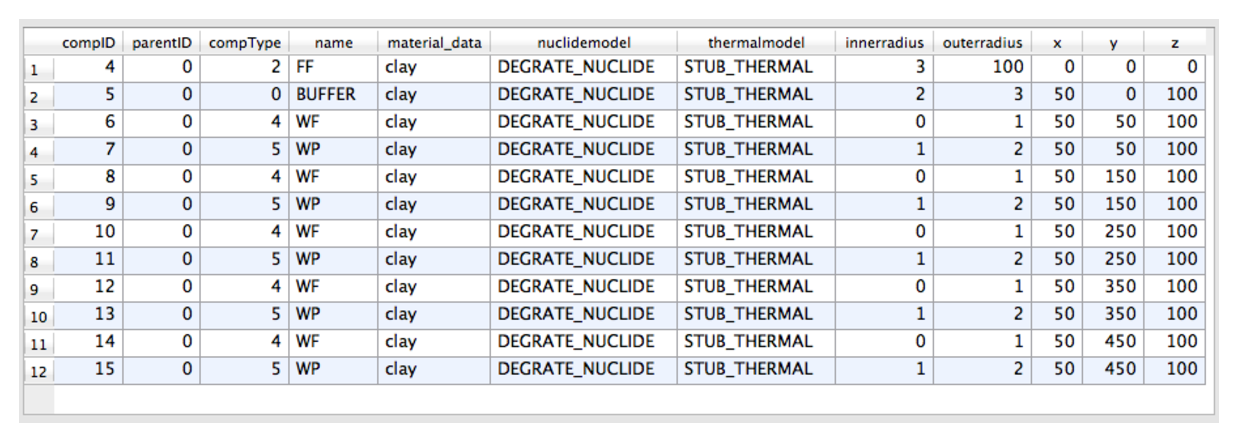
\includegraphics[width=\textwidth]{./chapters/paradigm/comp_table.eps}
      \caption[An example \Cyder output table of component parameters.]{An example of the \Cyder component parameters table recorded for provenance in the cyclus.sqlite database.}
      \label{fig:comp_table}
    \end{center}
  \end{figure}

  \begin{figure}[htbp!]
    \begin{center}
      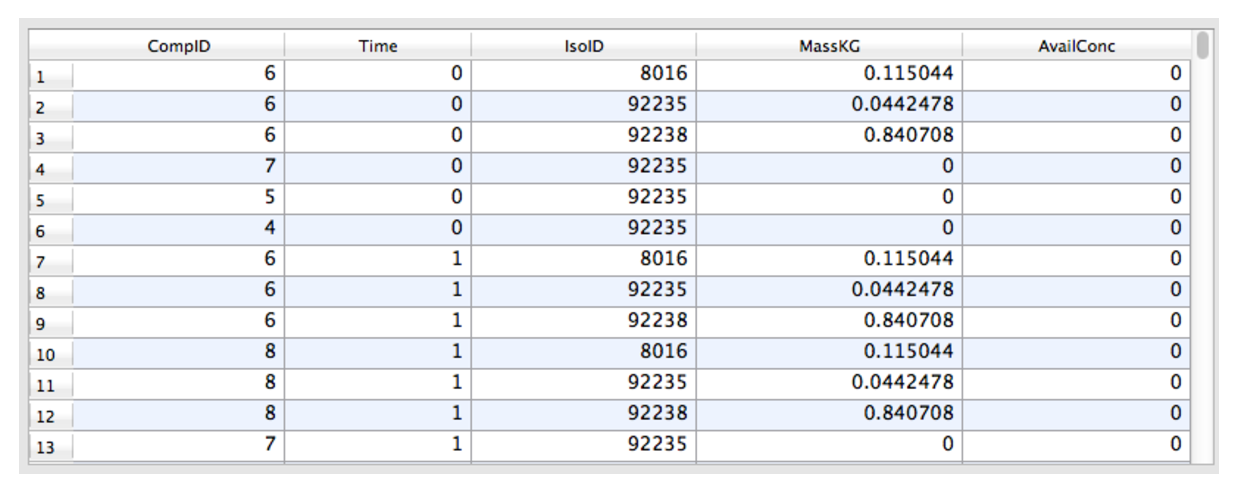
\includegraphics[width=\textwidth]{./chapters/paradigm/cont_table.eps}
      \caption[An example \Cyder output table of contaminant history.]{An example of the \Cyder contaminants table in the cyclus.sqlite database.}
      \label{fig:cont_table}
    \end{center}
  \end{figure}
